% Chapter 1

\chapter[Motivation and Background]
{Motivation and Background} % Main chapter title

\label{Chapter1} % For referencing the chapter elsewhere, use \ref{Chapter1} 

%----------------------------------------------------------------------------------------






% Define some commands to keep the formatting separated from the content 
\newcommand{\keyword}[1]{\textbf{#1}}
\newcommand{\tabhead}[1]{\textbf{#1}}
\newcommand{\code}[1]{\texttt{#1}}
\newcommand{\file}[1]{\texttt{\bfseries#1}}
\newcommand{\option}[1]{\texttt{\itshape#1}}

%----------------------------------------------------------------------------------------

\section[Quantum info processing and Qubit candidates]{Quantum info processing and Qubit candidates}


%----------------------------------------------------------------------------------------

\section[Silicon vacancy as a Qubit candidate]{Silicon vacancy as a Qubit candidate}

%\FloatBarrier
%\begin{figure}[h]
%\centering
%\includegraphics[width=0.7\linewidth]{Figures/pic/WP_20160921_20_40_25_Pro_LI}
%\caption{}
%\label{fig:wp20160921204025proli}
%\end{figure}
%\FloatBarrier

%\begin{figure}[h]
%\centering
%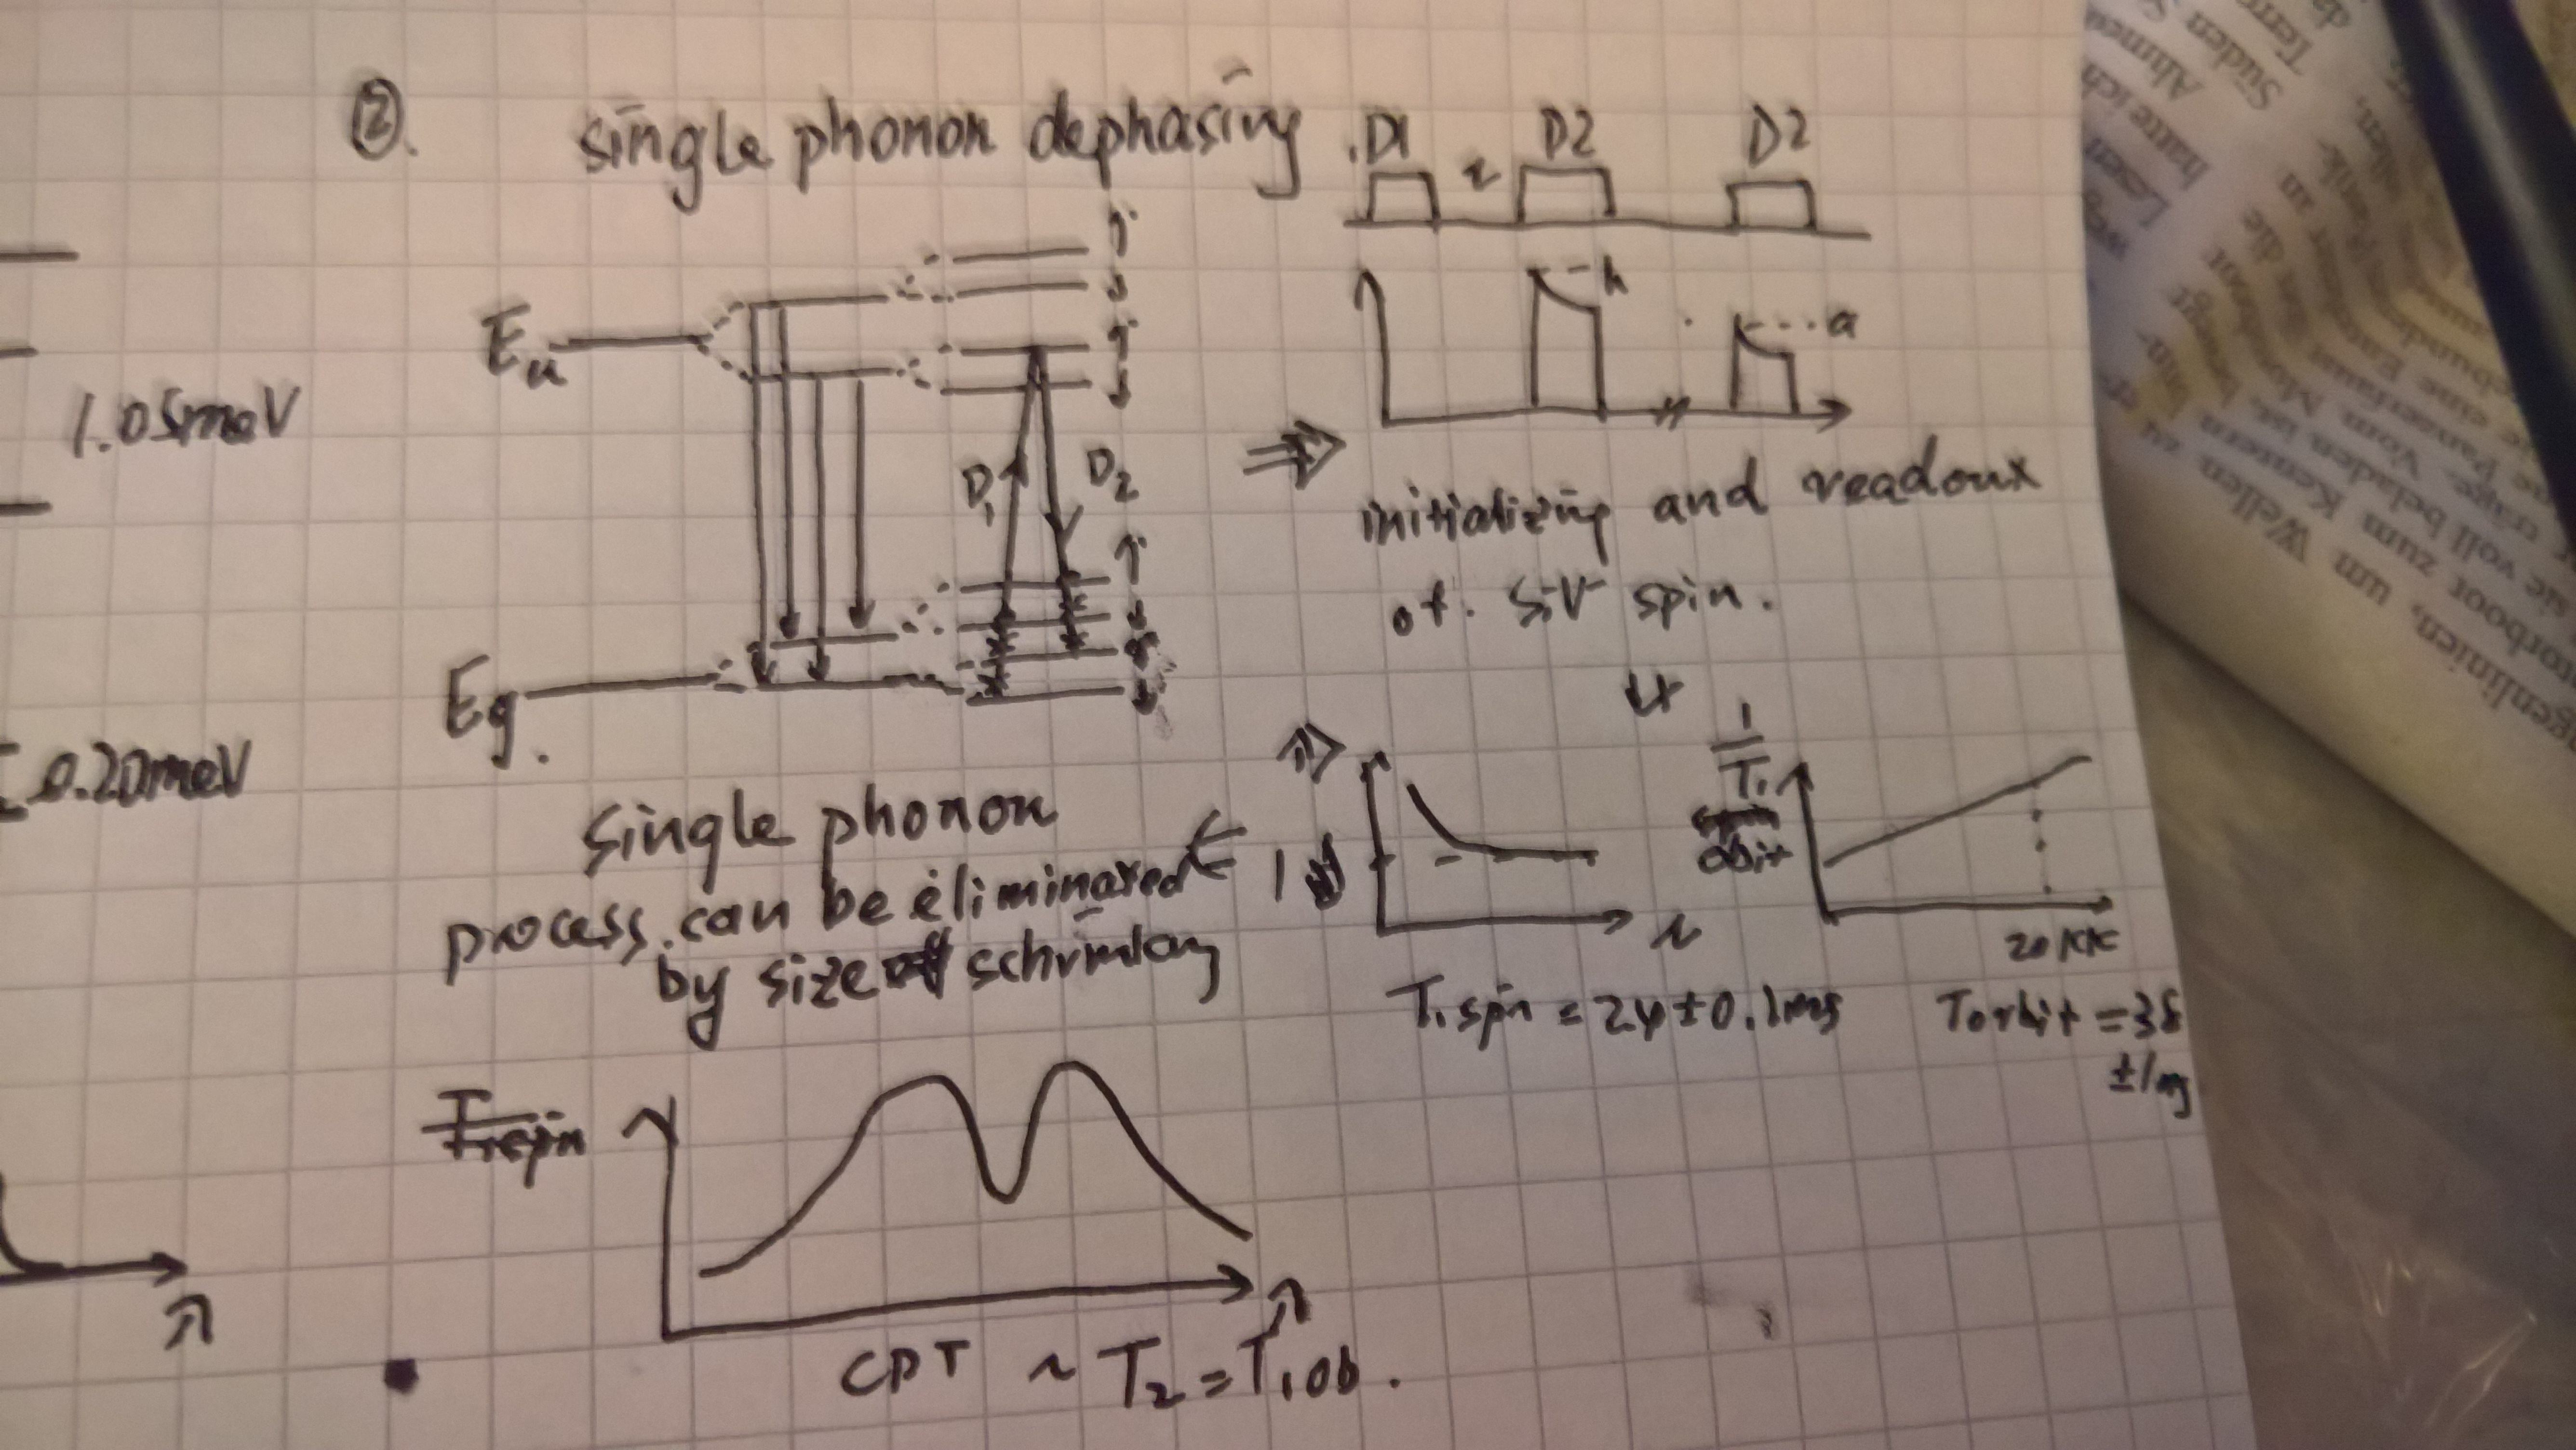
\includegraphics[width=0.7\linewidth]{Figures/pic/WP_20160921_20_40_32_Pro_LI}
%\caption{}
%\label{fig:wp20160921204032proli}
%\end{figure}
%\FloatBarrier

%----------------------------------------------------------------------------------------

\section[Silicon vacancies in nanodiamonds]{Silicon vacancies in nanodiamonds}
%\FloatBarrier
%\begin{figure}[h]
%\centering
%\includegraphics[width=0.7\linewidth]{Figures/pic/WP_20160921_20_40_48_Pro_LI}
%\caption{}
%\label{fig:wp20160921204048proli}
%\end{figure}
%\FloatBarrier
%----------------------------------------------------------------------------------------

\section[Motivation of the thesis, unsolved problem]{Motivation of the thesis, unsolved problem}
%\FloatBarrier
%\begin{figure}[h]
%	\centering
%	\includegraphics[width=0.7\linewidth]{Figures/pic/WP_20160921_20_40_42_Pro_LI}
%	\caption{}
%	\label{fig:wp20160921204042proli}
%\end{figure}
%\FloatBarrier
